\documentclass[11 pt]{article}

\usepackage
{
 listings, %Code listing
 hyperref, %Add hyperlink
 xcolor, %Color using package
 tcolorbox, %Text boxing
 imakeidx, %Indexing in alphabatical
 authblk, %Multiple author and affiliation
 pgfplots
}

\title{Geeks for Geeks problem discussion}
\author[1]
{
 Sofiullah Iqbal Kiron\\
 Mail: \href{mailto:sofiul.k.1023@gmail.com}{sofiul.k.1023@gmail.com}
}
\author[2]{\\Muhammad Ali Nirob}
\affil[1]{BSMRSTU, Department of CSE}
\affil[2]{Markazul Suffah, Madani}
\date{10 April, 2020}

\lstset
{
 language=C++,
 backgroundcolor=\color{black!15},
 stringstyle=\color{red},
 commentstyle=\color{green!80},
 keywordstyle=\color{blue},
 showstringspaces=false,
 basicstyle=\tiny,
 numbers=left,
 numberstyle=\tiny\color{orange},
 rulecolor=\color{green},
 captionpos=b
}

\renewcommand*\contentsname{Fulfilment}
\makeindex[columns=3, title=INDEX]

\begin{document}

\pagecolor{gray}
\maketitle
\pagebreak
\pagecolor{white}
\tableofcontents

\section{Is Binary Number Multiple of 3}
Problem Link: \href{https://practice.geeksforgeeks.org/problems/is-binary-number-multiple-of-3/0/#comment-4557555035}{LINK}

\subsection{My solution}
A number\index{number} will be divisible by 3 when the sum of all digits of this number is divisible by 3. Means, if sum of digits of a number is divisible by 3, the number is divisible by 3. School concept, COOL.
\\
It's a long processing method, not efficient.

\subsubsection{Algorithm}

\begin{tcolorbox}
\begin{enumerate}

\item Take a binary number string "s"
\item Create a Add() function for add two string
\item Create another function for returning power of 2 by string namely Pow2()
\item convert it to decimal, digit by digit, store in another string named "deci";
\item All apart of deci add to "decimal" string.
\item Create a function for give 'long long int' sum of "decimal"
\item If sum of all digits are divisible by 3, then the given number is divisible by 3, return true value, 1.\\Else return false, 0.

\end{enumerate}
\end{tcolorbox}

\subsubsection{Code}

\begin{lstlisting}

#include<iostream>
#include<algorithm>
#define lli long long int
using namespace std;

void Swap(string &s1, string &s2)
{
    string temp;
    temp = s1;
    s1 = s2;
    s2 = temp;
}

string Add(string s1, string s2)
{
    string result;
    int cs, carry=0;
    if(s1.size()<s2.size())
    {
        Swap(s1, s2);
    }
    int c1, c2;
    c1 = s1.size();
    c2 = s2.size();
    reverse(s1.begin(), s1.end());
    reverse(s2.begin(), s2.end());
    for(int i=c2; i<c1; i++)
    {
        s2.push_back('0');
    }
    for(int i=0; i<c1; i++)
    {
        cs = (s2[i]-'0')+(s1[i]-'0')+carry;
        result.push_back(cs%10+'0');
        carry=cs/10;
    }
    if(carry)
    {
        result.push_back(carry+'0');
    }
    reverse(result.begin(), result.end());

    return result;
}

string Pow2(int n)
{
    if(n==0)
    {
        return "1";
    }
    else if(n==1)
    {
        return "2";
    }
    string a = "2";
    int i;
    for(i=1; i<n; i++)
    {
        a = Add(a, a);
    }

    return a;
}

string bin_To_deci(string s)
{
    string decimal="0", deci;
    lli i, j;
    for(i=s.size()-1, j=0; i>=0; i--, j++)
    {
        if(s[i]=='1')
        {
            deci=Pow2(j);
            decimal=Add(decimal, deci);
        }
    }

    return decimal;
}

lli digit_sum(string s)
{
    lli sum = 0;
    string ss = bin_To_deci(s);
    for(int i=0; i<ss.size(); i++)
    {
        sum+=(ss[i]-'0');
    }
    return sum;
}

bool isM3(string s)
{
    if(digit_sum(s)%3==0)
    {
        return true;
    }
    else
    {
        return false;
    }
}

int main()
{
    int t;
    cin >> t;
    while(t--)
    {
        string s;
        cin >> s;
        if(isM3(s)==true)
        {
            cout << true << endl;
        }
        else
        {
            cout << false << endl;
        }
    }
}

\end{lstlisting}

\subsection{Geeks official solution}
Link: \href{https://www.geeksforgeeks.org/write-an-efficient-method-to-check-if-a-number-is-multiple-of-3/}{Write an Efficient Method to Check if a Number is Multiple of 3}.
\\
There is a pattern in the binary representation of the number. If A: sum of odd places bits, B: sum of even places bits; (A-B) mod 3 is equal to 0; then the number is divisible by 3;

\subsubsection{Proof of this method by number theory}
Let us consider a 4 digit binary number: $abcd$\\
Separate digits by place value. (Binary is 2 based number)\\
$
abcd = 2^3a+2^2b+2c+d\\
= 8a+4b+2c+d\\
= (9a-a)+(3b+b)+(3c-c)+d\\
= (9a+3b+3c)-a+b-c+d\\
= (9a+3b+3c)+{(b+d)-(a+c)}\\
$
Here $(9a+3b+3c)$ is divisible by $3$.
\\
So we can say that, the number will be divisible by $3$ if and only if $(iff)$, difference of sum of odd place bits and sum of even place bits is divisible by $3$.
\\
Considering one thing, there is no effect that how many $0$ bits we add for processing. So, if we count only "true" bit, that is enough.

\subsubsection{Algorithm}

\begin{tcolorbox}

\begin{enumerate}

\item Take a binary string namely "bs"
\item Calculate size of string;
\item If size is $1$:
 \begin{enumerate}
  \item If bs is equal to "0", return "true"
  \item Else, return "false"
 \end{enumerate}
\item Else:
\begin{enumerate}

\item Count or sum odd place non-zero bits, store in a variable namely A
 \begin{itemize}
 \item Write a for loop, initialize to bs.size()-1, decrement two by two, if current character is '1', increment A
 \item When loop variable becomes 0, over.
 \end{itemize}
\item Count or sum even place non-zero bits, store in a variable namely B
\item When loop variable becomes 0, over.
 \begin{itemize}
 \item Write a for loop, initialize to bs.size()-2, decrement two by two, if current character is '1', increment B
 \end{itemize}
\item If $(A-B) mod$ $3$ is equal to $0$, return "true"
\item Else return "false"

\end{enumerate}
\end{enumerate}
\end{tcolorbox}

\subsubsection{Code}

\begin{lstlisting}
#include<iostream>
#define mod %
using namespace std;

bool isM3(string s)
{
    if(s.size()==1)
    {
        if(s=="0")
        {
            return true;
        }
        else
        {
            return false;
        }
    }
    int i, A, B;
    for(i=s.size()-1, A=0; i>=0; i-=2)
    {
        if(s[i]=='1')
        {
            A++;
        }
    }
    for(i=s.size()-2, B=0; i>=0; i-=2)
    {
        if(s[i]=='1')
        {
            B++;
        }
    }
    if((A-B) mod 3 == 0)
    {
        return true;
    }
    else
    {
        return false;
    }
}

int main()
{
    int T;
    cin >> T;
    while(T--)
    {
        string bs;
        cin >> bs;
        if(isM3(bs)) /*No equal statement means,
                     if (true or non-zero)*/
        {
            cout << true << endl;
        }
        else
        {
            cout << false << endl;
        }
    }
}

\end{lstlisting}

\section{Contiguous subarray with largest sum}
Given an array, we need to find a subarray of this such as, sum of all elements of this array must be largest from another subarrays.For implement this, here are many algorithm with $O(n^6), O(n^3), O(n^2)$ but Kadane's algorithm is more efficient thats complexity is linear, $O(n)$. Ow, it's so simple. So let's get started\dots
\\Problem \href{https://practice.geeksforgeeks.org/problems/kadanes-algorithm/0}{source}.
\subsection{Kadane's algorithm}
\begin{tcolorbox}
\begin{itemize}
\item Declaring two variable, 
\end{itemize}
\end{tcolorbox}

\section{Majority Element}
Problem source is \href{https://practice.geeksforgeeks.org/problems/majority-element/0/}{here}.
\subsection{My Approach}
This is the matter of sorrow that, my approach is not accepted, showing time limit exit, because its time complexity gonna be $O(n^2)$.
\subsubsection{Algorithm}
\begin{tcolorbox}
\begin{enumerate}
 \item Count frequency of each elements and store in another array.
 \item Search in count array for major purpose.
 \item If: found, print the array and break.
 \item Else: loops over, print -1.
\end{enumerate}
\end{tcolorbox}
\subsubsection{Code}
\begin{lstlisting}[caption=Majority Element 1'st code, frame=shadowbox, rulesepcolor=\color{green!70}]
using namespace std;

int main()
{
    int t;
    cin >> t;
    while(t--)
    {
        int n, i, major;
        bool major_exist=false;
        cin >> n;
        major=n/2;
        int arr[n];
        for(i=0; i<n; i++)
        {
            cin >> arr[i];
        }
        for(i=0; i<n; i++)
        {
            if(count(arr, arr+n, arr[i])>major)
            {
                major_exist=true;
                cout << arr[i] << endl;
                break;
            }
        }
        if(major_exist==false)
        {
            cout << "-1" << endl;
        }
    }
}

\end{lstlisting}
So, it can be said simply, my approach is a f*****g approach.

\subsection{Solution by sorting}
Now we take approach from \href{https://www.geeksforgeeks.org/majority-element/}{geeks}.\\
Time complexity for this approach $O(n\log(n))$.\\
\begin{center}
\begin{tabular}{c c}
$n$ & $O(n\log(n))$\\
$3$ & $1.43136376416$\\
$5$ & $3.49485002168$
\end{tabular}
\end{center}
So, we can easily say that, this approach will take least time.
\\Auxiliary space $O(n)$.
\subsubsection{Algorithm}
\begin{tcolorbox}
\begin{enumerate}
 \item Declare \begin{tcolorbox}[colframe=red!50!white]
$major = \frac{size of array}{2}$.
\end{tcolorbox}
 \item Declare \begin{tcolorbox}[colframe=red!50!white]
bool major\_exist = false;
\end{tcolorbox}
 \item Sort the array and create two variable "count" and "previous".\begin{tcolorbox}[colframe=red!50!white]
count = 1;
\end{tcolorbox}
 \item Traverse array from start to end.
 \item If current element is equal to the previous element, increase count by one.
 \item When \begin{tcolorbox}[colframe=red!50!white]
count $>$= major+1;
\end{tcolorbox}
change value of major\_exist to true and print the current value, then break.
 \item If major\_exist till false then print -1.
 \item Over.
\end{enumerate}
\end{tcolorbox}

\pagebreak
\subsubsection{Code}
\begin{lstlisting}[caption=Majority Element $2'nd$ code, frame=shadowbox, rulesepcolor=\color{green!70}]
#include<bits/stdc++.h>
using namespace std;

int main()
{
    int t;
    cin >> t;
    while(t--)
    {
        int n, i, c=1, major;
        bool major_exist = false;
        cin >> n;
        major=n/2;
        int arr[n];
        for(i=0; i<n; i++)
        {
            cin >> arr[i];
        }
        sort(arr, arr+n);
        for(i=0; i<n; i++)
        {
            if(arr[i]==arr[i+1])
            {
                c++;
            }
            else
            {
                c=1;
            }
            if(c>=major+1)
            {
                major_exist=true;
                cout << arr[i] << endl;
                break;
            }
        }
        if(major_exist==false)
        {
            cout << "-1" << endl;
        }
    }
}
\end{lstlisting}

\section{Leaders in an array}
\href{https://practice.geeksforgeeks.org/problems/leaders-in-an-array/0/}{Link}\\
First, me approach uses two nested loop. That's why I got Time Limit Exceed. So, when got TIME LIMIT EXCEED, try to overcome nested loop. It causes increase order of time complexity. Try to use another STL Or simple loops but not nested.

\pagebreak
\subsection{Geeks Hint}
\subsubsection{Process}
Geeks hint was:\\
\tcbset{colback=pink!5!white, colframe=green!75!black}
\begin{tcolorbox}[arc = 6 mm, outer arc = 1 mm]
Scan all the elements from right to left in array and keep track of maximum till now. When maximum changes it’s value, print it.
\end{tcolorbox}
\subsubsection{My code by hints}
\begin{lstlisting}[caption=Leaders in an array]
#include<bits/stdc++.h>
using namespace std;

int main()
{
    int t;
    cin >> t;
    while(t--)
    {
        int n, i, j;
        list<int> L;
        cin >> n;
        int arr[n];
        for(i=0; i<n; i++)
        {
            cin >> arr[i];
        }
        int maxx=-1;
        for(i=n-1; i>=0; i--)
        {
            if(arr[i]>=maxx)
            {
                L.push_front(arr[i]);
                maxx=arr[i];
            }
        }
        list<int> :: iterator it;
        for(it=L.begin(); it!=L.end(); it++)
        {
            cout << *it << " ";
        }
        cout << endl;
    }
}
\end{lstlisting}

\subsubsection{Picture Run From \href{https://www.geeksforgeeks.org/leaders-in-an-array/}{Geeks}}
\begin{center}
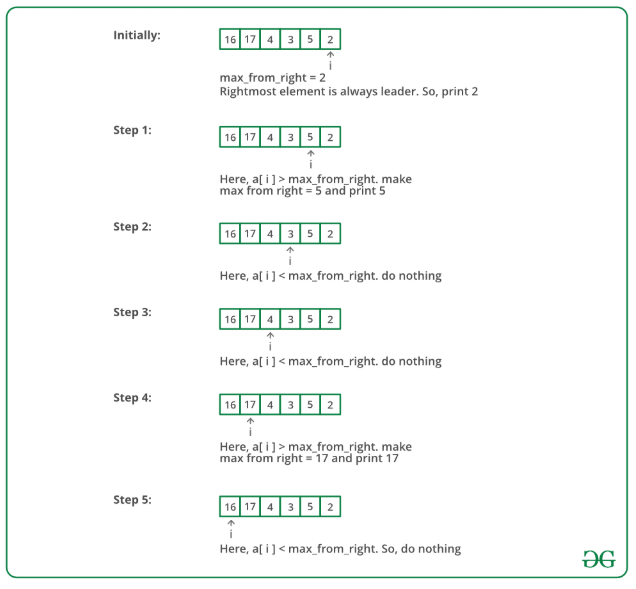
\includegraphics[width=240 pt]{Majority element picture run.png}
\end{center}

\subsubsection{Geeks official code}
\begin{lstlisting}
#include <bits/stdc++.h>
using namespace std;

long long a[10000000];
vector<long long>v;

int main()
{
   long long t;
   cin >> t;
   while (t--)
   {
       long long n;
       cin >> n;
       for(long long i =0;i<n;i++)
       {
           cin >> a[i];
       }
       long long max = a[n-1];
       for(long long i =n-1; i>=0; i--)
       {
           if(a[i] >= max)
           {
               max = a[i];
               v.push_back(max);
           }
       }
       reverse(v.begin(), v.end());
       for(auto it = v.begin(); it!=v.end(); it++)
       {
           cout << *it << " ";
       }
       v.clear();
       cout << endl;
   }
}
\end{lstlisting}

\begin{center}
\begin{tcolorbox}[size=minimal,auto outer arc,
width=2.1cm,octogon arc,
colback=red,colframe=white,colupper=white,
fontupper=\fontsize{7mm}{7mm}\selectfont\bfseries\sffamily,
halign=center,valign=center,
square,arc is angular]
OVER
\end{tcolorbox}
\end{center}

\printindex

\end{document}